\paragraph*{}\note{Любая наука включает в себя предмет исследований, методы исследований и ученых, которые этими исследованиями занимаются}

\paragraph*{}\gls{fzrsc} -- это наука о процессах, происходящих в растительном организме: почвенное, воздушное и гетеротрофное питание, синтез, транспорт и распад веществ, рост и развитие, движения растений, взаимодействие с патогенами, реакции на неблагоприятные факторы внешней среды. 


\paragraph*{}\gls{fzrsc} занимается процессами, происходящими на разных уровнях организации: молекулярном, субклеточном, клеточном, тканевом, органном, организменном и биоценотическом. Однако надо всегда иметь в виду, что в растении все процессы на любом уровне организации взаимосвязаны. Изменение какого-либо процесса сказывается на всей жизнедеятельности организма.

\subsection*{История развития знаний о физиологии растения}

\paragraph*{1634}  Я.Б. Ван Гельмонт (\ris \ref{ris_1} а) в своей книге сделан вывод о том, что вода используется для построения органической массы растения. В большинстве учебников становление физиологии растений как самостоятельной науки относят к 18 веку.

%%%%%%%%%%%%%%%%%%%%%%%%%%%%%%%%%%%%%%%%%%%%%%%%%%%%%%%%%%%%%%%%%%%%%%%%%%%%%%%%%%%%%%%%%%%%%%%%%%%%%%%%%%% 
%\begin{figure}
%  \centering
%       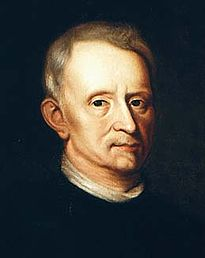
\includegraphics[width=0.5\linewidth]{pictures/gelmont}
%\caption{Я.Б. Ван Гельмонт}
%\label{gelmont}
%\end{figure}
%%%%%%%%%%%%%%%%%%%%%%%%%%%%%%%%%%%%%%%%%%%%%%%%%%%%%%%%%%%%%%%%%%%%%%%%%%%%%%%%%%%%%%%%%%%%%%%%%%%%%%%

\paragraph*{1727} г. С. Гейлс (\ris \ref{ris_1} б) установил, что движение воды по растению вызывают корневое давление и транспирация. 

%%%%%%%%%%%%%%%%%%%%%%%%%%%%%%%%%%%%%%%%%%%%%%%%%%%%%%%%%%%%%%%%%%%%%%%%%%%%%%%%%%%%%%%%%%%%%%%%%%%%%%%%%%% 
%\begin{figure}
%  \centering
%       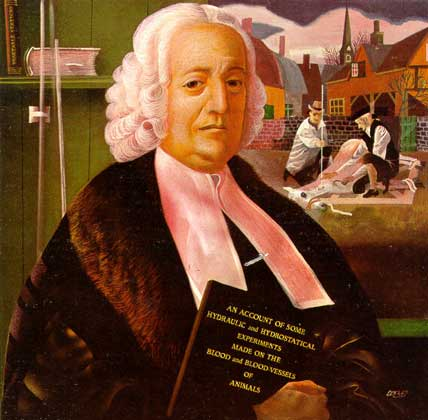
\includegraphics[width=0.5\linewidth]{pictures/geils}
%\caption{С. Гейлс}
%\label{geils}
%\end{figure}
%%%%%%%%%%%%%%%%%%%%%%%%%%%%%%%%%%%%%%%%%%%%%%%%%%%%%%%%%%%%%%%%%%%%%%%%%%%%%%%%%%%%%%%%%%%%%%%%%%%%%%%

\begin{figure}[h]
\begin{minipage}[h]{0.49\linewidth}
\center{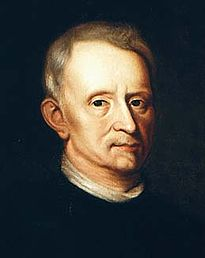
\includegraphics[width=0.7\linewidth]{pictures/gelmont} \\ а) Я.Б. Ван Гельмонт}
\end{minipage}
\hfill
\begin{minipage}[h]{0.49\linewidth}
\center{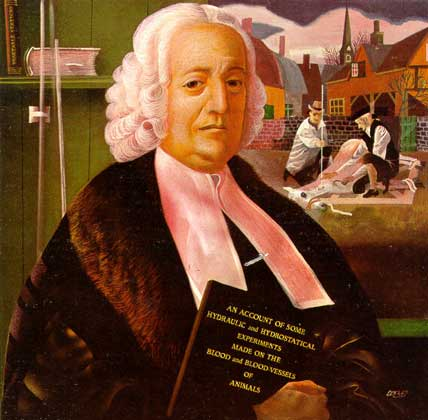
\includegraphics[width=0.9\linewidth]{pictures/geils} \\ б) С. Гейлс}
\end{minipage}
%\caption{Зависимость сигнала от шума для данных.}
\label{ris_1}
\end{figure}

%%%%%%%%%%%%%%%%%%%%%%%%%%%%%%%%%%%%%%%%%%%%%%%%%%%%%%%%%%%%%%%%%%%%%%%%%%%%%%

\paragraph*{1771} г. Дж. Пристли (\ris \ref{ris_2} а) открыл способность зеленых растений выделять на свету кислород.

%%%%%%%%%%%%%%%%%%%%%%%%%%%%%%%%%%%%%%%%%%%%%%%%%%%%%%%%%%%%%%%%%%%%%%%%%%%%%%%%%%%%%%%%%%%%%%%%%%%%%%%%%%% 
%\begin{figure}
%  \centering
%       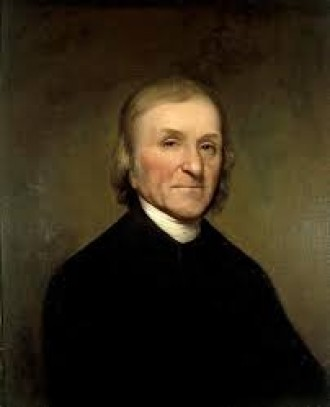
\includegraphics[width=0.5\linewidth]{pictures/pristli}
%\caption{С. Гейлс}
%\label{pristli}
%\end{figure}
%%%%%%%%%%%%%%%%%%%%%%%%%%%%%%%%%%%%%%%%%%%%%%%%%%%%%%%%%%%%%%%%%%%%%%%%%%%%%%%%%%%%%%%%%%%%%%%%%%%%%%% 

\paragraph*{1782} г. Ж. Сенебье (\ris \ref{ris_2} б) назвал поглощение $СО_{2}$ на свету <<углекислотным дыханием>>.  

%%%%%%%%%%%%%%%%%%%%%%%%%%%%%%%%%%%%%%%%%%%%%%%%%%%%%%%%%%%%%%%%%%%%%%%%%%%%%%%%%%%%%%%%%%%%%%%%%%%%%%%%%%% 
%\begin{figure}
%  \centering
%       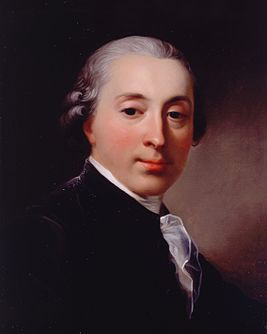
\includegraphics[width=0.5\linewidth]{pictures/senebier}
%\caption{Ж. Сенебье}
%\label{senebier}
%\end{figure}
%%%%%%%%%%%%%%%%%%%%%%%%%%%%%%%%%%%%%%%%%%%%%%%%%%%%%%%%%%%%%%%%%%%%%%%%%%%%%%%%%%%%%%%%%%%%%%%%%%%%%%% 

%%%%%%%%%%%%%%%%%%%%%%%%%%%%%%%%%%%%%%%%%%%%%%%%%%%%%%%%%%%%%%%%%%%%%%%%%%%%%%%%%%%%%%%%%%%%%%%%%%%%%%%

\begin{figure}[h]
\begin{minipage}[h]{0.49\linewidth}
\center{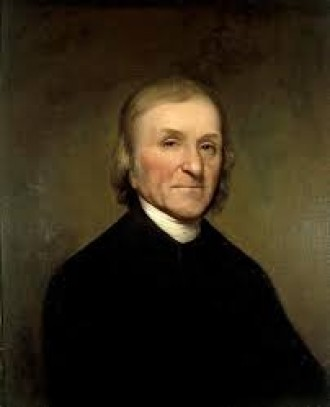
\includegraphics[width=0.8\linewidth]{pictures/pristli} \\ а) Пристли}
\end{minipage}
\hfill
\begin{minipage}[h]{0.49\linewidth}
\center{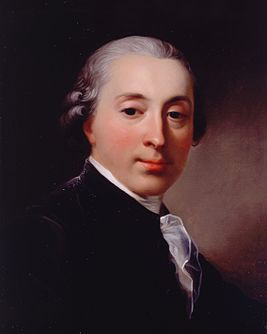
\includegraphics[width=0.8\linewidth]{pictures/senebier} \\ б) Ж. Сенебье}
\end{minipage}
%\caption{Зависимость сигнала от шума для данных.}
\label{ris_2}
\end{figure}

%%%%%%%%%%%%%%%%%%%%%%%%%%%%%%%%%%%%%%%%%%%%%%%%%%%%%%%%%%%%%%%%%%%%%%%%%%%%%%

\paragraph*{1797–1804} гг. Н. Т. Соссюр открыл дыхание у растений и рассчитал баланс газов при фотосинтезе. 

%%%%%%%%%%%%%%%%%%%%%%%%%%%%%%%%%%%%%%%%%%%%%%%%%%%%%%%%%%%%%%%%%%%%%%%%%%%%%%%%%%%%%%%%%%%%%%%%%%%%%%%%%%% 
\begin{figure}
  \centering
       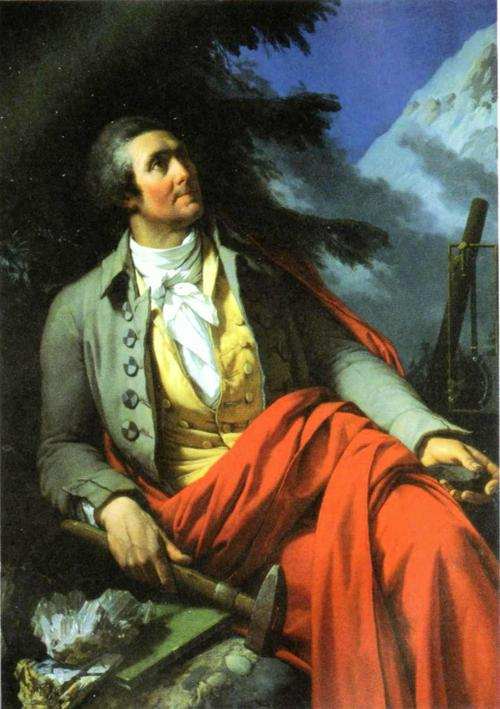
\includegraphics[width=0.35\linewidth]{pictures/saussr}
\caption{Н. Т. Соссюр}
\label{saussr}
\end{figure}
%%%%%%%%%%%%%%%%%%%%%%%%%%%%%%%%%%%%%%%%%%%%%%%%%%%%%%%%%%%%%%%%%%%%%%%%%%%%%%%%%%%%%%%%%%%%%%%%%%%%

\paragraph*{1800} г. Ж. Сенебье опубликовал пятитомный трактат <<Physiologie vegetale>>, в котором впервые определил физиологию растений как самостоятельную науку.

\subsection*{Цель и задачи физиологии растений}


\remember{Согласно современному определению \gls{fzrsc} изучает общие закономерности жизнедеятельности растительных организмов и является частью биологической науки}

\paragraph*{}Задачами физиологии на сегодняшний момент являются:

\begin{enumerate}

	\item изучение закономерностей жизнедеятельности растений (механизмы питания, роста, движения, размножения и др.); 
	\item разработка теоретических основ получения максимальных урожаев сельскохозяйственных культур; 
	\item разработка установок для осуществления процессов фотосинтеза в искусственных условиях.

\end{enumerate}

\paragraph*{}Физиология растений делится на две ветви: общую и прикладную. Задачей прикладной физиологии является изучение конкретных видов растений в конкретных экологических условиях.

\paragraph*{}Физиология растений служит основой для ряда других наук: агрохимии (наука о почвенном питании растений), растениеводства (наука о возделывании отдельных видов растений), селекции (наука о выведении новых сортов растений), фитопатологии (наука об инфекционных заболеваниях растений).

\subsection*{Место зеленого растения в природе и жизни человека}

\paragraph*{}Автотрофные растения Мирового океана за год способны превращать в органическое вещество 20–155 109 т углерода. Наземные растения фиксируют 16–24 109 т углерода. 
Только наземные растения накапливают ежегодно в форме углеводов 5-10 17 ккал. Даже 1 \% этой энергии достаточно для питания 5 млрд. человек. 